\section{Programme}
Für alle Module wurde ein gemeinsamer Programmcode geschrieben, bei dem mithilfe von einem \#define ausgewählt wird, welche Funktionen kompiliert und auf den jeweiligen Mikrocontroller geflasht werden. Die Wichtigsten dieser Funktionen werden in den Kapiteln \ref{Modulübergreifende Funktionen} bis \ref{Code der Eingabemodule} näher erläutert. Diese Herangehensweise wurde gewählt, da bei der Programmierung größerer Mengen von Mikrocontrollern die Wahrscheinlichkeit hoch ist, falsche Software zu flashen, wenn es mehrere sehr ähnliche Programme gibt. Zusätzlich ist die Entwicklung neuer Funktionen deutlich einfacher, da eine für alle Module notwendige Änderung nicht in mehrere Quelldateien angepasst werden muss.

\section{Modulübergreifende Funktionen}
\label{Modulübergreifende Funktionen}
Die Funktionen zum Lesen und Senden von Nachrichten müssen auf allen Modulen implementiert werden.

\subsection{Senden einer Nachricht}
In der übergeordneten Funktion sendMessage() wird zuerst die zu versendene Nachricht zusammengesetzt, und im Anschluss, wenn der Bus frei ist auf diesen geschrieben.

\lstinputlisting[firstline= 535, lastline=551,language = C++,frame=single,label=send(),caption=Senden einer Nachricht]{
	Kapitel/Programme/main.cpp}

Das Zusammensetzen der Nachricht erfolgt für jeden im Kapitel \ref{Datenbus} beschriebenen Teil der Busnachricht in einer eigenen Funktion, bei denen die einzelnen Bits an eine globale Nachricht angehängt werden. Folgend ein Beispiel der Adresse:

\lstinputlisting[firstline= 396, lastline=411,language = C++,frame=single,label=writeAdress(),caption=Adresse an globale Variable anhängen]{
	Kapitel/Programme/main.cpp}

Im Anschluss werden in die Nachricht mithilfe der Funktion writeBitstuffedMessage() die zusätzlichen Bits eingefügt, wenn mehr als drei gleichwertige Bits hintereinander folgen. 

\lstinputlisting[firstline= 495, lastline=523,language = C++,frame=single,label=send(),caption=Ausschnitt Bitstuffing]{Kapitel/Programme/main.cpp}

Um nun eine Nachricht auf den Bus zu schreiben, muss zunächst festgestellt werden, dass dieser gerade nicht beschrieben wird. Nur wenn dies der Fall ist, kann die Nachricht gesendet werden. Dabei wird zuerst der SOF gesendet, danach die Bitgestopfte Nachricht und im Anschluss das EOF.


\subsection{Empfangen einer Nachricht}
Solange ein Modul keine Nachricht senden möchte, hört es auf die Kommunikation auf dem Bus. Bei jedem empfangenen Start of Frame wird die Busfrequenz berechnet und gespeichert. \\
Dann wird solange eingelesen, bis das EOF empfangen wurde. 

\lstinputlisting[firstline= 314, lastline=340,language = C++,frame=single,label=recieve(),caption=Empfangen einer Nachricht]{
	Kapitel/Programme/main.cpp}

Im Anschluss wird die empfangene Bitgestopfte Nachricht in der Funktion 'decodeBitstuffedMessage' in die Originalnachricht zurückgewandelt, indem das Bit, welches auf eine Folge von 3 gleichwertigen Bits folgt aus der Nachricht entfernt wird.\\

\lstinputlisting[firstline= 232, lastline=253,language = C++,frame=single,label=recieve(),caption=decodeBitstuffedMessage()]{
	Kapitel/Programme/main.cpp}

Um die einzelnen Teile der Nachrichten zu extrahieren wird in der Funktion 'parseDecodedMessage' erst die Adresse und das COF ausgelesen, da die Länge dieser jeweils auf 3 Bit festgelegt ist und im Anschluss die Daten basierend auf dem Wert des COF extrahiert. Der Rest der Nachricht ist dann das CRC Feld. Alle Nachrichtenteile werden in je einer globalen Variable gespeichert. 

\lstinputlisting[firstline= 263, lastline=299,language = C++,frame=single,label=recieve(),caption=parseDecodedMessage()]{
	Kapitel/Programme/main.cpp}

Wenn die hier ermittelte Adresse mit der eigenen Adresse übereinstimmt, sowie die zyklische Redundanzprüfung erfolgreich war, werden die empfangenen Daten weiter verarbeitet, ansonsten wird die Nachricht ignoriert.  

\subsection{CRC}
Ein Teil der Nachricht ist die zyklische Redundanzprüfung (CRC). Es wurde eine CRC16 ... mit dem Polynom '0x1021' implementiert. Folgend ist die Berechnung der CRC Prüfsumme dargestellt:

\lstinputlisting[firstline= 137, lastline=153,language = C++,frame=single,label=recieve(),caption=crc16()]{
	Kapitel/Programme/main.cpp}

Um die Prüfsumme zu verifizieren, wurde zudem die Funktion 'verifyCrc16' implementiert. Hier werden die Daten schrittweise durch das festgelegte Polynom geteilt und geprüft ob ein Rest vorhanden ist. Ist dies der Fall wird die Nachricht einfach ignoriert.

\lstinputlisting[firstline= 155, lastline=172,language = C++,frame=single,label=recieve(),caption=verifyCrc16()]{Kapitel/Programme/main.cpp}

\newpage
\section{Controller Modul - Programmcode}
Das Controller Modul übernimmt die folgenden Aufgaben:
\begin{enumerate}
    \item Verwaltung der Adressvergabe an angeschlossene Module
    \item Abfrage nach neuen Daten der einzelnen Module
    \item Übermittlung dieser Daten über eine UART-Schnittstelle an den angeschlossenen Rechner
\end{enumerate}

\begin{figure}[H]
	\centering    
	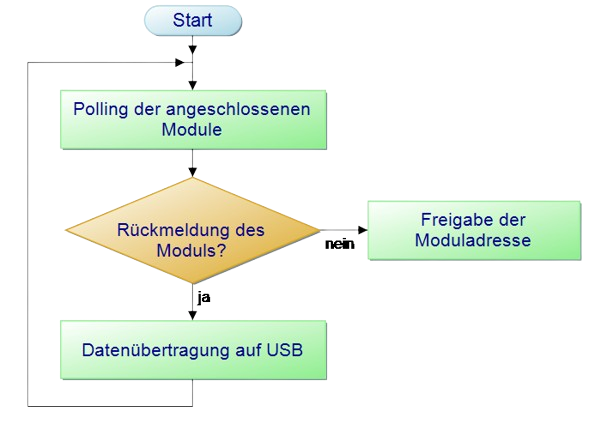
\includegraphics[width=.75\textwidth]{Bilder/pap_hauptmodul.png}
	\caption{Programmablauf Controller Modul}
	\label{Programm_Controller Modul}
\end{figure}
\textmd{
}

\subsection{Adressvergabe und Verwaltung}
Das Controller Modul speichert alle vergebenen Adressen zusammen mit den zugehörigen Funktionen sowie weiteren Variablen der jeweiligen Module in einer Liste von Structs. Diese Liste wird für das Polling der Teilnehmer verwendet, wodurch sichergestellt wird, dass ausschließlich die tatsächlich angeschlossenen Module abgefragt werden.\\


\lstinputlisting[firstline= 5, lastline=20,language = C++,frame=single,label=structDevice,caption=Struct device]{Kapitel/Programme/header.h}


Die jeweiligen Module haben keine festgelegte Adresse. Wenn diese also mit Spannung versorgt werden, warten sie auf die Adressvergabe des Controller Moduls. In der Polling Liste wird eine bestimmte Adresse (0x00) abgefragt, um festzustellen, ob ein neuer Teilnehmer an den Bus angeschlossen wurde. Wenn eine Rückmeldung auf diese Adresse festgestellt wird, dann enthält die nächste Nachricht die Adresse für den neuen Teilnehmer. In der Rückmeldung eines Moduls ist dessen Funktion hinterlegt. Diese Informationen werden in der Adressliste abgespeichert und das Gerät ab dem Zeitpunkt mit abgefragt.\\

\lstinputlisting[firstline= 704, lastline=734,language = C++,frame=single,label=newAdress(),caption= Zuweisen einer neuen Adresse]{Kapitel/Programme/main.cpp}

Wenn ein Modul nicht mehr über den Bus kommuniziert, wird dessen Adresse nach mehreren fehlgeschlagenen Versuchen (Timeout) aus der Polling-Liste entfernt und wieder den verfügbaren Adressen zugewiesen. Dadurch wird sichergestellt, dass alle aktiven Geräte schnellstmöglich vom Controller Modul abgefragt werden und Adressen für neu verbundene Geräte freigegeben werden. Die Anzahl der nicht Rückmeldungen wurde auf drei festgelegt, kann aber in den 'defines' des Controller Moduls angepasst werden.
\\

\lstinputlisting[firstline= 767, lastline=796,language = C++,frame=single,label=timeout(),caption=Timeout Funktion]{Kapitel/Programme/main.cpp}

Wenn keine Antwort eines Eingabemoduls in der vorgegebenen Wartezeit empfangen wird, wird der Timeout-Counter iteriert. Sobald dieser seinen Maximalwert erreicht, wird das Gerät nicht mehr abgefragt und dessen Adresse freigegeben.


\subsection{Abfrage neuer Daten}
Die Daten jedes Moduls werden einmal pro Durchlauf der Polling Liste abgefragt. Sobald neue Daten empfangen wurden, werden diese abgespeichert und dem angeschlossenen Computer über die UART-Schnittstelle übermittelt.\\

\lstinputlisting[firstline= 799, lastline=832,language = C++,frame=single,label=polling(),caption=Polling Funktion]{
	Kapitel/Programme/main.cpp}

\subsection{Übermittlung der Daten an den angeschlossenen Computer}
Sobald neue Daten von einem Modul empfangen worden sind, werden diese an den Computer übermittelt. Diese Kommunikation erfolgt über eine UART Schnittstelle und den auf dem PCB verbauten UART zu USB Bridge IC. Zu den übermittelten Daten wird neben der jeweiligen Funktion auch die zugehörige Adresse übermittelt, sodass die Daten nicht nur abhängig von der Funktion ausgewertet werden können, sondern auch mehrere gleiche Module voneinander unterschieden werden können.\\
Damit alle Busteilnehmer in das Input-Mapper Programm eingebunden und konfiguriert werden können, wird alle 10 Polling Durchläufe eine Liste aller Module einschließlich ihrer Funktion übermittelt. Diese Liste wird auch gesendet, sobald sich die Anzahl der Busteilnehmer ändert.\\
Zudem wird zur Ermittlung des COM-Ports an dem das Controller Modul an den PC angeschlossen alle 10 Polling Durchläufe ist ein festgelegter String (\glqq INIT
\grqq) übermittelt.
\lstinputlisting[firstline= 652, lastline=701,language = C++,frame=single,label=usb(),caption=Datenübertragung an den angeschlossenen Computer]{
	Kapitel/Programme/main.cpp}

\section{Code der Eingabemodule}
\label{Code der Eingabemodule}
Im Folgendem wird der Programm-Ablauf eines Eingabemoduls genauer beschrieben. Dieses Modul hat folgende Aufgaben:
\begin{enumerate}
    \item Anforderung einer Adresse bei Neustart
    \item Auswerten der Modulfunktion
    \item Übermitteln der Daten an das Controller Modul bei Anfrage
\end{enumerate}

\begin{figure}[H]
	\centering    
	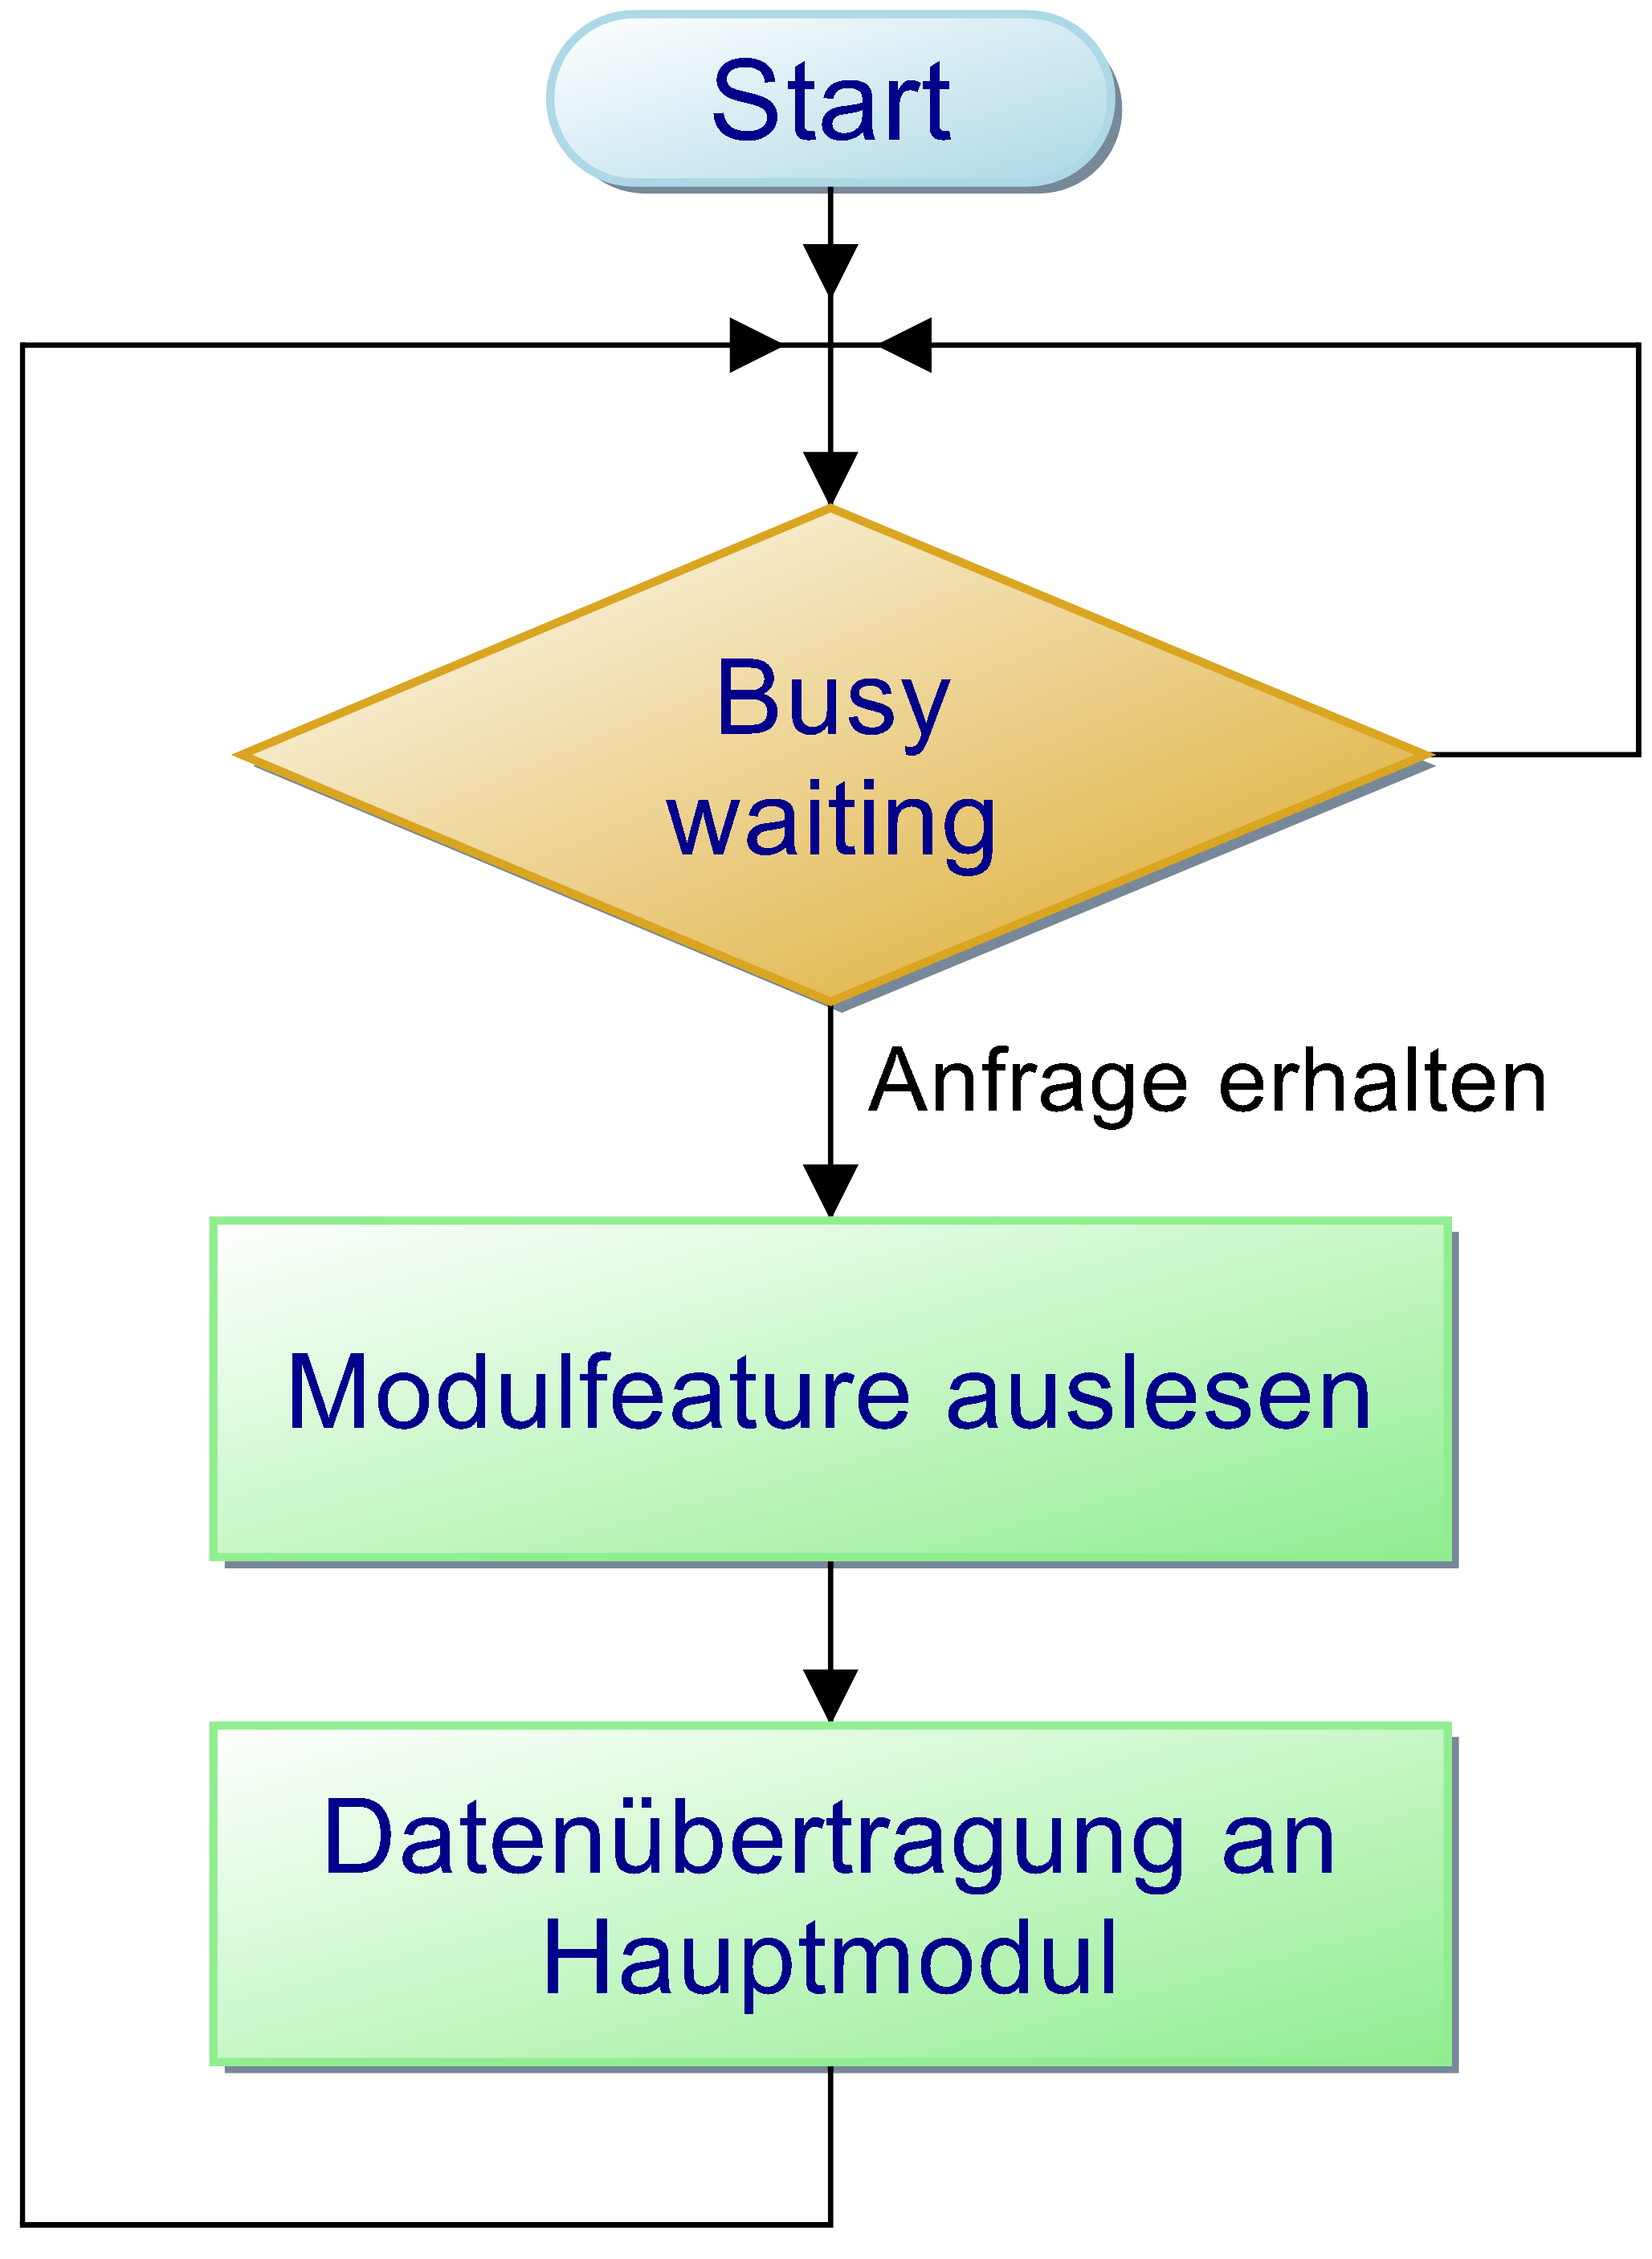
\includegraphics[width=.75\textwidth]{Bilder/pap_eingabemodul.png}
	\caption{Programmablauf eines Eingabemoduls}
	\label{Programm_Eingabemodul}
\end{figure}

\subsection{Anforderung einer Adresse}
Wenn einem Modul noch keine Adresse zugewiesen wurde und der Controller nach neuen Teilnehmern auf dem Bus sucht, antwortet das Modul mit einer Nachricht, in der seine Funktion in den übertragenen Daten enthalten ist. Anschließend übermittelt der Hauptcontroller eine neue Adresse an das Modul. Diese Adresse wird vom Modul gespeichert, sodass es danach ausschließlich auf diese Adresse reagiert.\\

\lstinputlisting[firstline= 582, lastline=595,language = C++,frame=single,label=getAdress(),caption=Anfordern einer Adresse]{
	Kapitel/Programme/main.cpp}


\subsection{Auswertung der Modulfunktion}
Die Auswertung der Modulfunktion ist abhängig von der jeweiligen Funktion des Moduls und kann daher nicht verallgemeinert werden.\\
Im Fall des Tastatur-Moduls werden die Tasten nur dann ausgewertet, wenn der Controller das Modul abfragt. Anschließend werden die Daten übermittelt. Für diese Auswertung wurde eine allgemeine Funktion geschrieben, die jedoch für jedes Modul spezifisch angepasst werden muss.\\

\lstinputlisting[firstline= 597, lastline=626,language = C++,frame=single,label=myfunction(),caption=Beispiel Funktion Tastaturmodul]{Kapitel/Programme/main.cpp}

\subsection{Übermittlung der Daten an das Controller-Modul}
Sobald eine Anfrage des Controller Moduls an die Adresse des Eingabemoduls empfangen wird, übermittelt dieses die Information der Modulfunktion. Im Falle der Tastatur wären dies die zurzeit gedrückten Tasten. Dabei nimmt jede gedrückte Taste ein Byte der Daten ein.


